% Copyright 2020 by Junwei Wang <i.junwei.wang@gmail.com>
%
% This file may be distributed and/or modified under the
% conditions of the LaTeX Project Public License, either version 1.3c
% of this license or (at your option) any later version.
% The latest version of this license is in
%   http://www.latex-project.org/lppl.txt

\documentclass[compress]{beamer}
\usepackage[utf8]{inputenc}

\usepackage[english]{babel}
\usepackage{metalogo}
\usepackage{listings}
\usepackage{fontspec}
\usepackage{tikz}
\usetikzlibrary{arrows, petri, topaths}
\usepackage{tkz-berge}
\usepackage{caption}
\usepackage{subcaption}
\usepackage{amsmath}
\usepackage{amsthm}
\usepackage{amssymb}
\usepackage{mathtools}
\usepackage{siunitx}
\usepackage{csquotes}

\usepackage{algorithm}
\usepackage{algpseudocode}

\lstset{basicstyle=\scriptsize}

\usetheme{Nord}
\setmainfont{Yanone Kaffeesatz}
\setsansfont{Andika New Basic}
\setmonofont{DejaVu Sans Mono}

\AtBeginSection[]
{
  \begin{frame}[c,noframenumbering,plain]
    \tableofcontents[sectionstyle=show/hide,subsectionstyle=show/show/hide]
  \end{frame}
}

%\AtBeginSubsection[]
%{
%  \begin{frame}[c,noframenumbering,plain]
%    \tableofcontents[sectionstyle=show/hide,subsectionstyle=show/shaded/hide]
%  \end{frame}
%}

\title{Competitive Programming Workshop}
\subtitle{Day 2}
\author{Giacomo Fabris, Francesco Lotito}
\institute{University of Trento}
\date{2020-07-15}

\begin{document}

\begin{frame}[plain,noframenumbering]
    \maketitle
\end{frame}

\begin{frame}[plain,noframenumbering]
    \tableofcontents
\end{frame}

\section{Previous week's contest}

\begin{frame}{Problem C - hello}{}
    \begin{figure}
        
\includegraphics[height=0.8\textheight]{meme1}
    \end{figure}
\end{frame}

\begin{frame}{Problem F - inflation}
    Greedy matching between canisters and balloons: assign the smallest canister to the smallest balloon.

    \begin{enumerate}
        \item Sort input vector;
        \item loop from 1 to N, compute the minimum inflation ratio, quick fail if the canister is too big.
    \end{enumerate}
\end{frame}

\begin{frame}{Problem E - kleptography}
    We receive as input a ciphertext $b$ of length $m$ and the last $n$ characters of the plaintext $a$. We shall decipher the whole plaintext.
    The key $k$ is composed of an initialization vector of length $n$, then, $k[n + i] = a[i]$.
    The encryption function is: $b[i] = (a[i] + k[i]) (\text{mod } 26)$

    \bigskip
    We see that:
    \begin{align*}
        k[i]             & = b[i] - a[i] (\text{mod } 26)           \\
        a[i]             & = k[i + n]                               \\
        \Rightarrow a[i] & = (b[i + n] - a[i + n]) (\text{mod } 26) \\
    \end{align*}
\end{frame}

\begin{frame}{Problem D - jabuke}
    Area calculation is straightforward - just compute it using the provided formula.

    To test whether a point $P \coloneqq (x, y)$ is inside or outside the triangle $ABC$ with vertices $A \coloneqq (x_A, y_A)$, $\dots$, you have (at least) two options:
    \begin{enumerate}
        \item sum areas of triangles $ABP$, $ACP$, $BCP$; see if it matches area of triangle $ABC$
        \item compute the implicit function of rays passing through $AB$, $BC$, $AC$; $P$ is inside the triangle if $r_{AB}(x_P, y_P) \cdot r_{AB}(x_C, y_C) \geq 0$, and the same shall hold for $r_{BC}$ w.r.t. vertex $A$ and $r_{AC}$ w.r.t. vertex $B$.
    \end{enumerate}
\end{frame}

\begin{frame}{Problem B - divisors}{\#1}
    Definition of combinations:
    \begin{equation*}
        \binom{n}{k} \coloneqq \frac{n!}{k! (n - k)!}
    \end{equation*}

    Always remember this handy formula:
    \begin{equation*}
        \left (\frac{n}{k} \right )^k \leq \binom{n}{k} \leq \left ( \frac{en}{k} \right ) ^k
    \end{equation*}

    Combinations grow very fast, you cannot compute them directly.
\end{frame}

\begin{frame}{Problem B - divisors}{\#2}
    The easy way to do this:
    \begin{enumerate}
        \item factorize each term separately; all numbers are $\leq 431$ --- precompute all primes up to 431 using e.g. Sieve of Erathostenes;
        \item memorize the exponent $n$ of each prime number (sum all exponents of the numerator, subtract those of the denominator);
        \item every prime number could not be chosen, or chosen up to $n$ times.
    \end{enumerate} \pause

    \medskip
    Some optimization tricks may be necessary to make this solution pass the time limit, e.g.:
    \begin{itemize}
        \item load a static array / constexpr containing the prime numbers, do not execute the sieve at runtime;
        \item note that the first $k$ terms of the factorial are always simplified and therefore shall not be factorized;
        \item w.r.t. the previous suggestion, remember that $\binom{n}{k} = \binom{n}{n-k}$
    \end{itemize}
\end{frame}

\begin{frame}{Problem B - divisors}{\#3}
    The clever way to do this: open Wikipedia and search for \textbf{Legendre's formula}.

    It will speed-up calculation for this problem.
\end{frame}

\section{Basic concepts}

\begin{frame}{Big O notation}
\begin{figure}
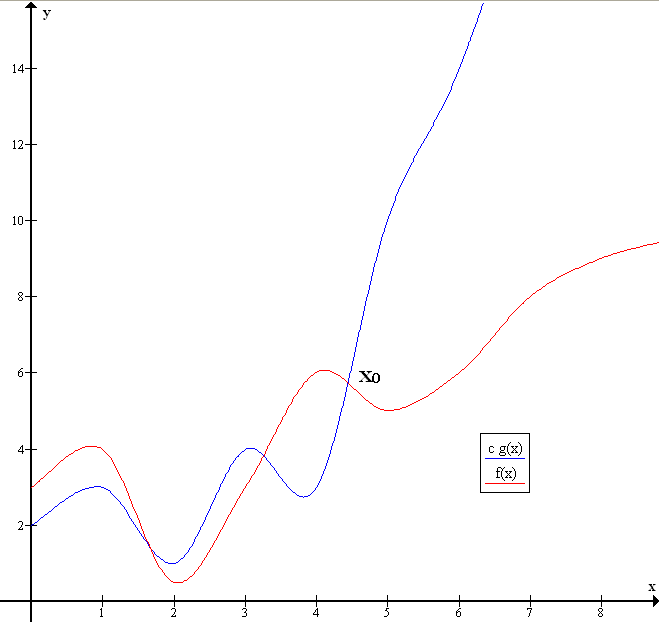
\includegraphics[height=0.8\textheight]{Big-O-notation}
\caption{ $f(x) \in \mathcal{O}(g(x))$ as there exists $c > 0$ and $x_0$ such that $f(x) \leq cg(x) ~~ \forall x \geq x_0$.}
\end{figure}
\end{frame}


\begin{frame}{Aggregate analysis}
    We may obtain tighter upper bounds if we know the frequency of worst-case executions.
    
    Aggregate analysis evaluates the upper bound averaging on multiple executions.

\end{frame}

\section{STL wonderland}

\begin{frame}{std::vector}
    \begin{block}{Rationale}
        Elements are indexed and stored contiguously. Size of underlying array is automatically handled.
    \end{block}\pause

    %\setbeamercolor{block title}{use=structure,fg=white,bg=cyan!75!black}
    \begin{block}{Interface}
        \begin{itemize}
            \item $[~]$ operator - access element at index (note: undefined behaviour if index $>$ underlying array size) - $\mathcal{O}(1)$
            \item $push\_back(elem)$ - append element to the end - amortized $\mathcal{O}(1)$
            \item $assign(n, elem)$ - initialize vector of size $n$ assigning each cell the element $elem$. Second parameter is optional - $\mathcal{O}(n)$ Note: same arguments of constructor.
        \end{itemize}
    \end{block}
\end{frame}

\begin{frame}[fragile]{std::vector usage}
    \begin{block}{Sort vector}
        \begin{lstlisting}
std::sort(v.begin(), v.end());
\end{lstlisting}
    \end{block}
    \begin{block}{Sort vector of custom type}
        \begin{lstlisting}
typedef pair<int, int> ii;
bool mycomp(const ii a, const ii b) {
    return a.first < b.first;
}
//...
std::sort(v.begin(), v.end(), mycomp);
\end{lstlisting}
    \end{block}
\end{frame}
\begin{frame}[fragile]{std::vector usage}
    \begin{block}{Sort vector of custom type, lambda flavour}
        \begin{lstlisting}
std::sort(v.begin, v.end(), [](const ii a, const ii b) {
    return a.first < b.first;
});
\end{lstlisting}
    \end{block}
    \begin{block}{Initialize DP matrix}
        \begin{lstlisting}
v.assign(N, vector<int>(N, -1));
\end{lstlisting}
    \end{block}
\end{frame}

\begin{frame}{std::queue, std::stack}
    \begin{block}{Rationale}
        Queues and stacks are really nothing more than a vector with a (slightly) different interface.
    \end{block}
\end{frame}

\begin{frame}{std::priority\_queue}
    \begin{block}{Rationale}
        A queue in which elements are sorted. If two elements have the same priority, then FIFO.

        Implemented (by default) as a std::vector and a heap.
    \end{block}\pause

    \begin{block}{Interface}
        \begin{itemize}
            \item $empty()$: test empty - $\mathcal{O}(1)$
            \item $push(elem)$: insert element - amortized $\mathcal{O}(\log n)$ \\ ($\mathcal{O}(\log n)$ heap insertion + amortized $\mathcal{O}(1)$ vector push)
            \item $front()$: access top element - $\mathcal{O}(1)$
            \item $pop()$: remove top element - $\mathcal{O}(1)$
        \end{itemize}
    \end{block}
\end{frame}

\begin{frame}[fragile]{std::priority\_queue usage}
    \begin{block}{Dijkstra's prioq}
        Use $std::greater$, which is the default, reverse-order comparator for built-in types (works also with $std::pair$!)
        \begin{lstlisting}
typedef pair<int, int> ii;
//...
priority_queue<ii, std::vector<ii>, std::greater<ii>> pq;
pq.push(ii(0, 0));
\end{lstlisting}
    \end{block}
\end{frame}

\begin{frame}{std::set, std::unordered\_set}
    \begin{block}{Rationale}
        Containers that store unique values, and which allow for fast retrieval of individual elements based on their value.
        \begin{itemize}
            \item std::set are ordered (trees!)
            \item std::unordered\_set are unordered (hash maps!)
            \item std::multiset and std::unordered\_multiset may have non-unique values
        \end{itemize}
    \end{block}\pause

    \begin{block}{Interface}
        \begin{itemize}
            \item $find(elem)$: find element - returns an iterator (set::end if not found)
            \item $insert(elem)$: inserts element (if exists and set is not multi, no change)
        \end{itemize}
    \end{block}
\end{frame}

\begin{frame}{std::set, std::unordered\_set usage}
    \begin{block}{Notes on complexity}
        \begin{itemize}
            \item Average case, insertion in a set is $\mathcal{O}(log~n)$, accessing an element is $\mathcal{O}(log~n)$.
            \item Average case, insertion in an unordered\_set is $\mathcal{O}(1)$, accessing an element is $\mathcal{O}(1)$
            \item $\to$ in competitive programming always use unordered\_set if order does not matter and you do not need to access elements sequencially
        \end{itemize}
    \end{block}
\end{frame}

\begin{frame}[fragile]{Set operations}
    \begin{block}{Set intersection}
        \begin{lstlisting}
unordered_set<int> sa, sb, si;
set_intersection(sa.begin(),sa.end(),sb.begin(),sb.end(),
    std::inserter(si,si.begin()));
\end{lstlisting}

Similarly, there is also

        And also: $set\_difference$, $set\_simmetric\_difference$, $set\_union$.

        Complexity: linear in the cost of insertion and access to the set ($\mathcal{O}(N)$ if unordered, $\mathcal{O}(N \log N)$ if ordered)
    \end{block}
\end{frame}

\begin{frame}{std::map, std::unordered\_map}
    \begin{block}{Rationale}
        \begin{itemize}
            \item A set for the keys and an ancillary data structure storing the valueassociated to each key.
            \item We have std::map, std::unordered\_map, std::multimap, std::unordered\_multimap
        \end{itemize}
    \end{block}
\end{frame}

\begin{frame}{}
    \begin{block}{Interface}
        Not that different from a set, note:
        \begin{itemize}
            \item In a $map<K, V>$ you shall insert $std::pair<K, V>$. Using a typedef is probably the fastest way to do it.
            \item You can access directly a value using the $[ ]$ operator, passing the desired key between brackets. While this may seem fancy, note that it has a strange behaviour: if you access a key which is not in the map, a new element is inserted, regardless whether an r-value has been passed! (In that case, constructor default will be used)
            \item $Rightarrow$ test if a key is in the map using $map.find() != map.end()$ (it returns the iterator of the element)
        \end{itemize}
    \end{block}

\end{frame}
\section{Union-Find Disjoint Set}

\begin{frame}{Intro}
    STL is nice, its data structures are general-purpose and have a wide range of applications.
    
    However, in CP, sometimes (often) it is necessary to use more tailored data structures.
    
    Today we will see one of the many well known DS, not implemented in the STL: the UFDS.
\end{frame}

\begin{frame}{Definition}
    A Union-Find Disjoint Set is a data structure which models a \textbf{collection of disjoint sets}.

    As the name suggests, the following operations are usually implemented:
    \begin{itemize}
        \item initialize the UFDS with $n$ sets $\lbrace 1 \rbrace, \lbrace 2 \rbrace, \dots, \lbrace n \rbrace$ in $\mathcal{O}(n)$\pause
        \item \textbf{union}: merge two sets of the UFDS in (almost) $\mathcal{O}(1)$\pause
        \item \textbf{find}: determine which set an item belongs to / determine if two items belong to the same set in $\mathcal{O}(1)$
    \end{itemize}
    \bigskip

    Using the STL (e.g. vector of unordered sets?) these operations would be slower!    
\end{frame}

\begin{frame}{Idea}
    The UFDS data structure is stored as a forest, i.e. every disjoint set is a tree, where the root, the \enquote{representative} element, is just one element of the set.

    The forest is memorized as a vector $V$ of $n$ integers. $V[i]$ contains the parent of the tree of the element $i$; if $i$ is a root then $V[i] = i$. When the UFDS is initialized, $V[i] = i~~\forall i$.

    \begin{figure}
        %\renewcommand*{\EdgeColor}{NordBlue}
%\renewcommand*{\VertexLineColor}{NordDarkBlack}
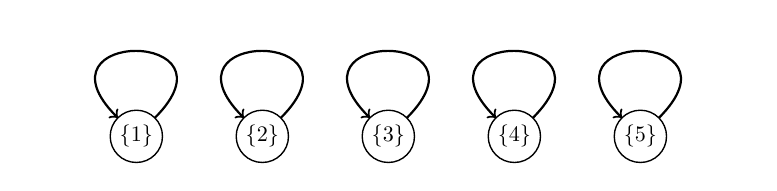
\begin{tikzpicture}[scale=0.8,transform shape]
    %\GraphInit[vstyle=Welsh]
    %\SetVertexNoLabel
    \SetGraphUnit{2}
    \Vertex[Math,L=\lbrace 1 \rbrace]{1}
    \EA[Math,L=\lbrace 2 \rbrace](1){2}
    \EA[Math,L=\lbrace 3 \rbrace](2){3}
    \EA[Math,L=\lbrace 4 \rbrace](3){4}
    \EA[Math,L=\lbrace 5 \rbrace](4){5}
    %\AddVertexColor{NordOrange}{1, 2, 3, 4, 5}
    %\AddVertexColor{NordBrightBlack}{1, 2, 3, 4, 5, 6}
    \Loop[dist=2cm,dir=NO,style={thick,->}](1)
    \Loop[dist=2cm,dir=NO,style={thick,->}](2)
    \Loop[dist=2cm,dir=NO,style={thick,->}](3)
    \Loop[dist=2cm,dir=NO,style={thick,->}](4)
    \Loop[dist=2cm,dir=NO,style={thick,->}](5)
\end{tikzpicture}
    \end{figure}
\end{frame}

\begin{frame}{Operations}
    \texttt{Root(x)}: return the representative node of the set in which $x$ is. Simple tree visit. \pause

    \bigskip
    \texttt{Union(x, y)}: merge the two trees which contain the element $x$ and $y$, which means, change the representative of $y$ to be $x$ (or the other way around). Heuristic improvement: perform the merge which minimizes the resulting depth.\pause

    \bigskip
    \texttt{Find(x, y)}: \texttt{Root(x) == Root(y)}
    
\end{frame}

\begin{frame}{Path compression}
    Whenever we find the representative (root) item of a disjoint set by traversing the tree from the leaves to the root, we can set the parent of all items traversed to point directly to the root.

    All subsequent find operations may be performed with single access to the vector $V$.
\end{frame}

\begin{frame}{Example}
    \begin{figure}
        %\renewcommand*{\EdgeColor}{NordBlue}
%\renewcommand*{\VertexLineColor}{NordDarkBlack}
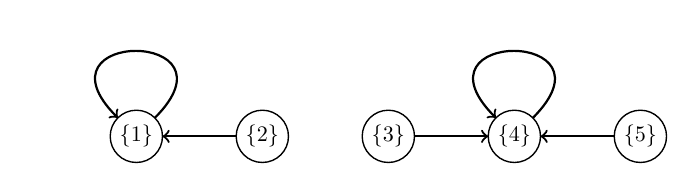
\begin{tikzpicture}[scale=0.8,transform shape]
    %\GraphInit[vstyle=Welsh]
    %\SetVertexNoLabel
    \SetGraphUnit{2}
    \Vertex[Math,L=\lbrace 1 \rbrace]{1}
    \EA[Math,L=\lbrace 2 \rbrace](1){2}
    \EA[Math,L=\lbrace 3 \rbrace](2){3}
    \EA[Math,L=\lbrace 4 \rbrace](3){4}
    \EA[Math,L=\lbrace 5 \rbrace](4){5}
    \Edge[style={thick,->}](2)(1)
    \Edge[style={thick,->}](5)(4)
    \Edge[style={thick,->}](3)(4)
    %\AddVertexColor{NordOrange}{1, 2, 3, 4, 5}
    %\AddVertexColor{NordBrightBlack}{1, 2, 3, 4, 5, 6}
    \Loop[dist=2cm,dir=NO,style={thick,->}](1)
    \Loop[dist=2cm,dir=NO,style={thick,->}](4)
\end{tikzpicture}
        \caption{Sets: $\lbrace \lbrace 1, 2 \rbrace, \lbrace 3, 4, 5 \rbrace \rbrace$}
    \end{figure}

    \begin{figure}
        %\renewcommand*{\EdgeColor}{NordBlue}
%\renewcommand*{\VertexLineColor}{NordDarkBlack}
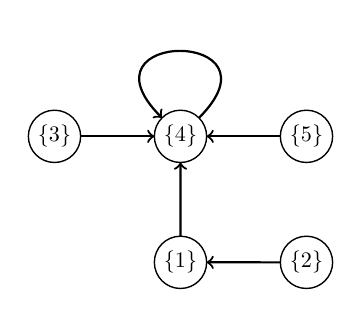
\begin{tikzpicture}[scale=0.8,transform shape]
    %\GraphInit[vstyle=Welsh]
    %\SetVertexNoLabel
    \SetGraphUnit{2}
    \Vertex[Math,L=\lbrace 4 \rbrace]{4}
    \EA[Math,L=\lbrace 5 \rbrace](4){5}
    \WE[Math,L=\lbrace 3 \rbrace](4){3}
    \SO[Math,L=\lbrace 1 \rbrace](4){1}
    \EA[Math,L=\lbrace 2 \rbrace](1){2}
    \Edge[style={thick,->}](2)(1)
    \Edge[style={thick,->}](5)(4)
    \Edge[style={thick,->}](3)(4)
    \Edge[style={thick,->}](1)(4)
    %\AddVertexColor{NordOrange}{1, 2, 3, 4, 5}
    %\AddVertexColor{NordBrightBlack}{1, 2, 3, 4, 5, 6}
    \Loop[dist=2cm,dir=NO,style={thick,->}](4)
\end{tikzpicture}
        \caption{\texttt{Union (2, 4)}}
    \end{figure}
\end{frame}

\begin{frame}{Example}
    \begin{figure}
        %\renewcommand*{\EdgeColor}{NordBlue}
%\renewcommand*{\VertexLineColor}{NordDarkBlack}
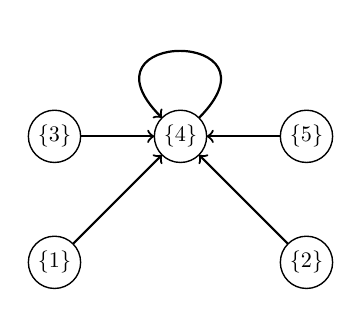
\begin{tikzpicture}[scale=0.8,transform shape]
    %\GraphInit[vstyle=Welsh]
    %\SetVertexNoLabel
    \SetGraphUnit{2}
    \Vertex[Math,L=\lbrace 4 \rbrace]{4}
    \EA[Math,L=\lbrace 5 \rbrace](4){5}
    \WE[Math,L=\lbrace 3 \rbrace](4){3}
    \SOWE[Math,L=\lbrace 1 \rbrace](4){1}
    \SOEA[Math,L=\lbrace 2 \rbrace](4){2}
    \Edge[style={thick,->}](2)(4)
    \Edge[style={thick,->}](5)(4)
    \Edge[style={thick,->}](3)(4)
    \Edge[style={thick,->}](1)(4)
    %\AddVertexColor{NordOrange}{1, 2, 3, 4, 5}
    %\AddVertexColor{NordBrightBlack}{1, 2, 3, 4, 5, 6}
    \Loop[dist=2cm,dir=NO,style={thick,->}](4)
\end{tikzpicture}
        \caption{Path compression after \texttt{Find (2, 4)}}
    \end{figure}
\end{frame}


\begin{frame}[plain,noframenumbering]{}
    Thanks!

    \bigskip
    Today's contest: \url{https://open.kattis.com/contests/ucen9t}
\end{frame}

\end{document}